\chapter{Introduzione}
Il lavoro svolto per l'esame di Metriche e Modelli di Internet ha posto l'interesse nell' analisi del comportamento di un sistema web al variare di alcune sue componenti. Nello specifico sono state condotte due tipi di analisi, la prima da un punto di vista \var{simulativo} mentre la seconda da un punto di vista \var{analitico}. Entrambe fanno riferimento ad una 
rappresentazione matematica del sistema reale(modello) denominata \var{rete di code}(QN, Queueing Network). Una QN tiene conto della contesa per le risorse del sistema e delle code che si generano in attesa del servizio. 
La soluzione analitica consente di risolvere mediante l’uso di formule e algoritmi una rete di code, ottenendo in questo modo i valori prestazionali desiderati. Tali valori possono altresì essere ottenuti emulando il comportamento del sistema attraverso una simulazione. 
La simulazione è realizzata mediante un programma in grado di mimare il funzionamento del sistema attraverso flussi di transazioni tra le varie risorse. I valori di performance sono ricavati dalle statistiche collezionate dal programma per ogni coda relativa a tali risorse. 
Per poter generare un modello di performance è necessario innanzitutto stilare un modello che rappresenti il workload, che nel caso specifico, è stato generato a partire da diverse distribuzioni rappresentanti più valori, come ad esempio il numero di richieste per sessione o la dimensione della pagina html richiesta. 
Per rendere più chiara l'idea al lettore, si presentano di seguito i requisiti del progetto.
\section{Requisiti del Progetto}
Si consideri il cluster di Server Web in figura \ref{schema1}. Il sistema è composto da un Web Switch che riceve le richieste dagli utenti e le distribuisce ad un set di N Server Web. Il Web Switch è connesso alla rete internet mediante il link L1. I Web Server e il Web Switch sono tra di loro connessi mediante la LAN L2. 
Ogni server è caratterizzato da una CPU, da uno o più dischi ed una scheda di rete (Iw2). La CPU dei server ha un tasso di servizio pari a 150 richieste al secondo (indipendentemente dal tipo di richieste). Il disco ha le seguenti caratteristiche: Seek Time 8.5ms, Controller Time 0.2ms, Rotational Speed 7200 RPM, transfer rate 100MB/sec, block size 2048 byte. 
Il Web Switch è caratterizzato da una CPU e da due scheda di rete (Is1 e Is2), una che lo connette alla rete L1 ed una che lo connette alla rete L2. 
La rete L2 è una rete Ethernet 1000Mbit/sec e sia i Web Server che il Web Switch sono ad essa connessi mediante delle schede di rete con un transfer rate di 1000Mbit/sec. 
\begin{figure}[H]
\begin{center}
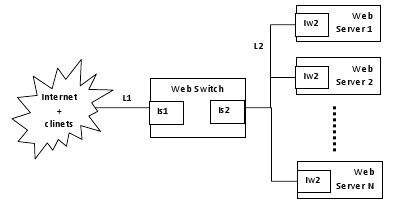
\includegraphics[scale=1.2]{etc/schema1.png}
\caption{Schema}
\label{schema1}
\end{center}
\end{figure}
Si suppone che il carico del sistema è caratterizzato come segue:
\begin{table}[H]
\begin{center}
\begin{tabular}{||c|c|c||}
\hline
Richieste 	&Gaussiana Inversa			&$X > 0; \mu = 3.86;$\\
per Sessione & 							&$\lambda = 9.46$\\
\hline
\hline
User Think Time				&Pareto		&$X \geq k; \alpha=1.4; k = 1$\\
\hline
Num. Oggetti 	&Pareto		&$X \geq k; \alpha=1.33; k = 2$\\
per Richiesta	&			&\\							
\hline
Dim. Pag. HTML	&LogNormale-Pareto	&$\mu = 7.63; \sigma = 1.001$ \\
					&					&$X \geq k; \alpha=1; k = 10240 (byte)$\\
\hline
Embedded Objects	&LogNormale			&$X > 0; \mu = 8.215; \sigma = 1.46$\\
\hline
\end{tabular}
\end{center}
\caption{specifiche}
\label{test_1}
\end{table}
Si chiede agli studenti di studiare il comportamento del sistema utilizzando un modello di simulazione e, fatta l’opportuna caratterizzazione del carico, mediante la risoluzione di un modello analitico. Nello specifico si chiede di: 
\begin{itemize}
	\item Dimensionare opportunamente il sistema per far si che sia in grado di sopportare un carico di 150 utenti al secondo con un utilizzazione massima della risorsa collo di bottiglia compresa tra il 65 ed il 70\%.
	\item Studiare le prestazioni del sistema al variare delle politiche di selezione dei server (ROUND ROBIN, RANDOM, LEAST LOADED) 
	\item Valutare che impatto ha sulle prestazioni del sistema l’introduzione di 
	\begin{enumerate}
		\item una scheda di rete addizionale per i web server (per la gestione separata delle richieste in ingresso ed in uscita)
		\item un link in uscita, dimensionato opportunamente, per lo smistamento delle risposte (Vedi fig. \ref{schema2}) 
	\end{enumerate}
	\item Valutare che impatto ha, sulle prestazioni del sistema, l’introduzione di un proxy server che offra un cache hit rate del 40\%.
\end{itemize}
\begin{figure}[H]
\begin{center}
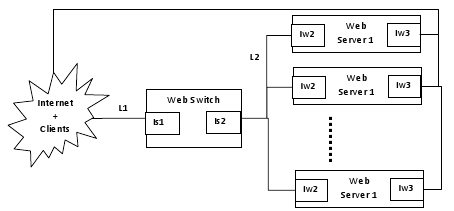
\includegraphics[scale=1.2]{etc/schema2.png}
\caption{Schema}
\label{schema2}
\end{center}
\end{figure}
\section{Approccio Adottato}
Si presenta di seguito un breve sunto dei passi che hanno consentito di realizzare il progetto (NON MI PIACE PER NIENTE, DA CORREGGERE), e che verranno affrontati nei capitoli successivi.
\begin{enumerate}
	\item Caratterizzazione del workload raggruppando i documenti in cluster in base alle loro dimensioni;
	\item Scelta delle risorse da modellare come centri di servizio
	\item Sviluppo della simulazione ed esecuzione di un set di simulazione per la stima dei parametri da modellare;
	\item Studio del transiente
	\item Esclusione del transiente dalla simulazione 
	\item Sviluppo ed esecuzione del modello analitico
\end{enumerate}
